\documentclass[notes, xcolor=dvipsnames]{beamer}    

\usetheme{Berkeley}

\setbeamertemplate{footline}[frame number]

\usepackage{amsmath}
\usepackage{inputenc}
\usepackage{graphicx}
\usepackage{hyperref}

\title{Constraint based scheduling of Weakly Consistent C programs for Reconfigurable Hardware}
\author{Akshay Gopalakrishnan}

\begin{document}

    \begin{frame}
        
        \maketitle

    \end{frame}

    \begin{frame}{Problem}

        \begin{itemize}
            \item Scheduling concurrent C programs for HLS. 
            \item When using atomics, scheduling can be incorrect. 
            \item Existing solution assumes no constraints on resources.
        \end{itemize}

    \end{frame}

    \begin{frame}{Current Approach}

        \begin{itemize}
            \item Introduce memory dependency edges to influence scheduling. 
            \item Map each thread to an independent H/W Accelerator.
            \item No constraints on resources. 
        \end{itemize}

    \end{frame}

    \begin{frame}{Proposed Solution: Sequentialize}

        \begin{itemize}
            \item Merge two or more concurrent threads to meet resource constraints. 
            \item Give the merged program to be synthesized by the same HLS tool. 
            \item Merging would also expose other thread-local optimizations in synthesis which may reduce clock cycles(why?).
        \end{itemize}

    \end{frame}

    \begin{frame}{Current Progress}
        \begin{itemize}
            \item Added shared memory accesses to coursework code base. 
            \item Added new dependency order to respect memory consistency rules.
            \item Modified scheduling algorithm of coursework to handle shared memory programs.
            \item Identified a good benchmark to showcase advantage of merging. 
        \end{itemize}
    \end{frame}

    \begin{frame}{Benchmark Programs}

        \begin{figure}
            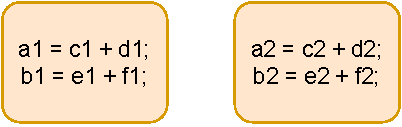
\includegraphics[scale=0.6]{Benchmark.pdf}
        \end{figure}

        \begin{itemize}
            \item Change any access above to shared one -- eg: c1-->cs.  
            \item Do this for all memory accesses -- total 4096 possibilitie -- giving us 4096 programs.
        \end{itemize}
        
    \end{frame}


    \begin{frame}{Test Example 0: No shared memory}
        
        \begin{figure}
            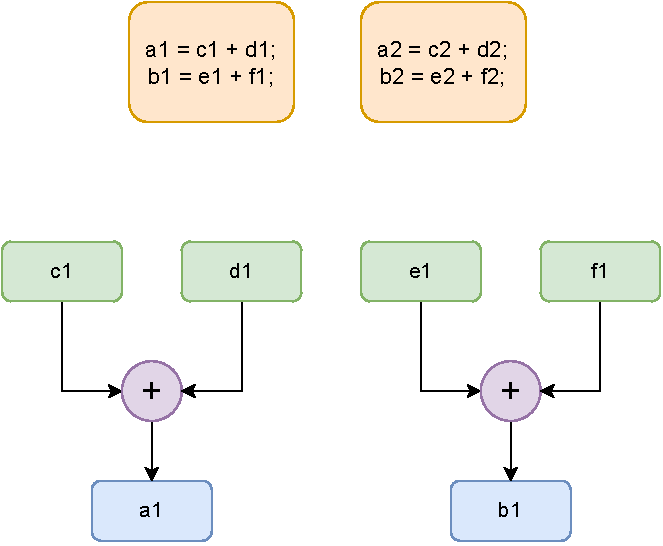
\includegraphics[scale=0.4]{NoSharedEx.pdf}
        \end{figure}

    \end{frame}

    \begin{frame}{Test Example 1: All Shared memory }

        T1;T2
        \begin{figure}
            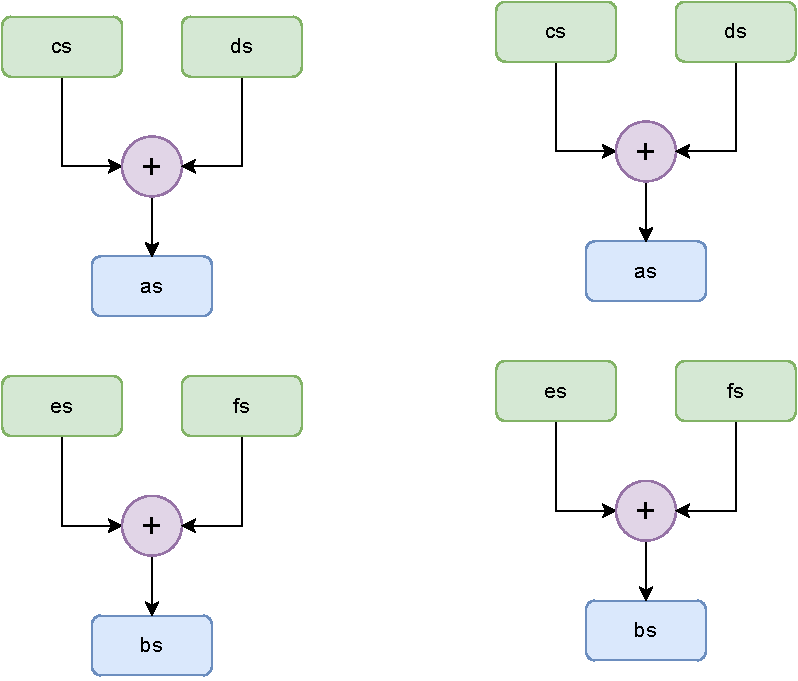
\includegraphics[scale=0.4]{AllSharedMerge.pdf}
        \end{figure}

    \end{frame}

    \begin{frame}{Test Example 2: Save Clock Cycles}

        T2;T1
        \begin{figure}
            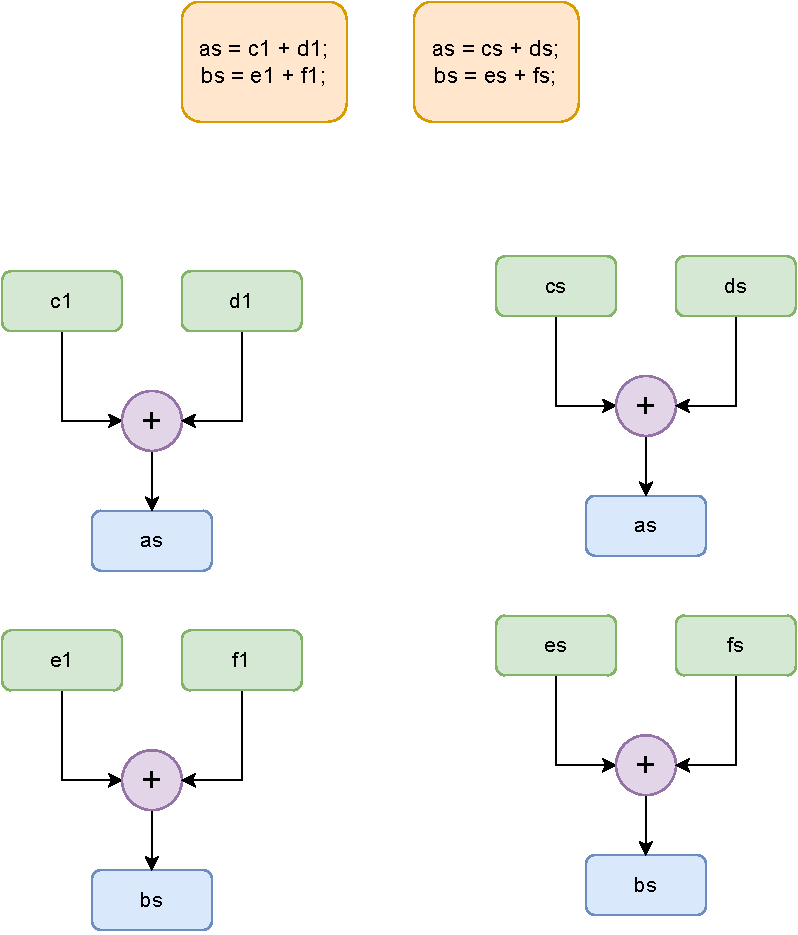
\includegraphics[scale=0.4]{PartialSharedMerge.pdf}
        \end{figure}


    \end{frame}

    \begin{frame}{Test Example 3: Save Both Clock Cycles and Resources}

        T1;T2
        \begin{figure}
            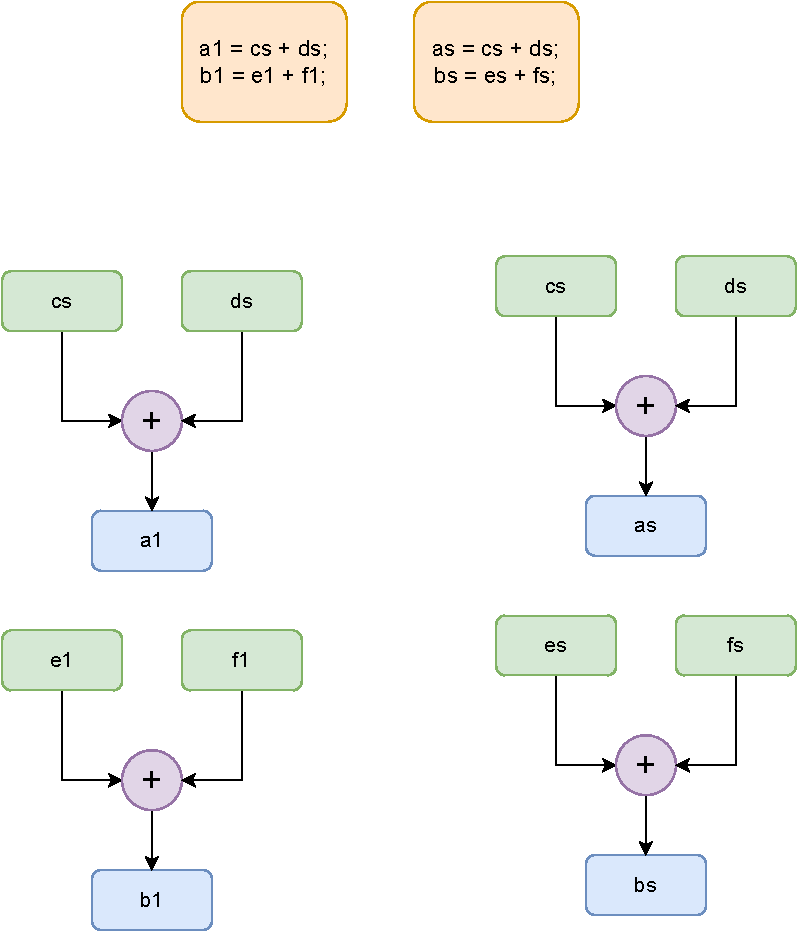
\includegraphics[scale=0.4]{PartialSharedMergeClkRes.pdf}
        \end{figure}

    \end{frame}

    \begin{frame}{Can do even better}

        T2-T1-T1-T2
        \begin{figure}
            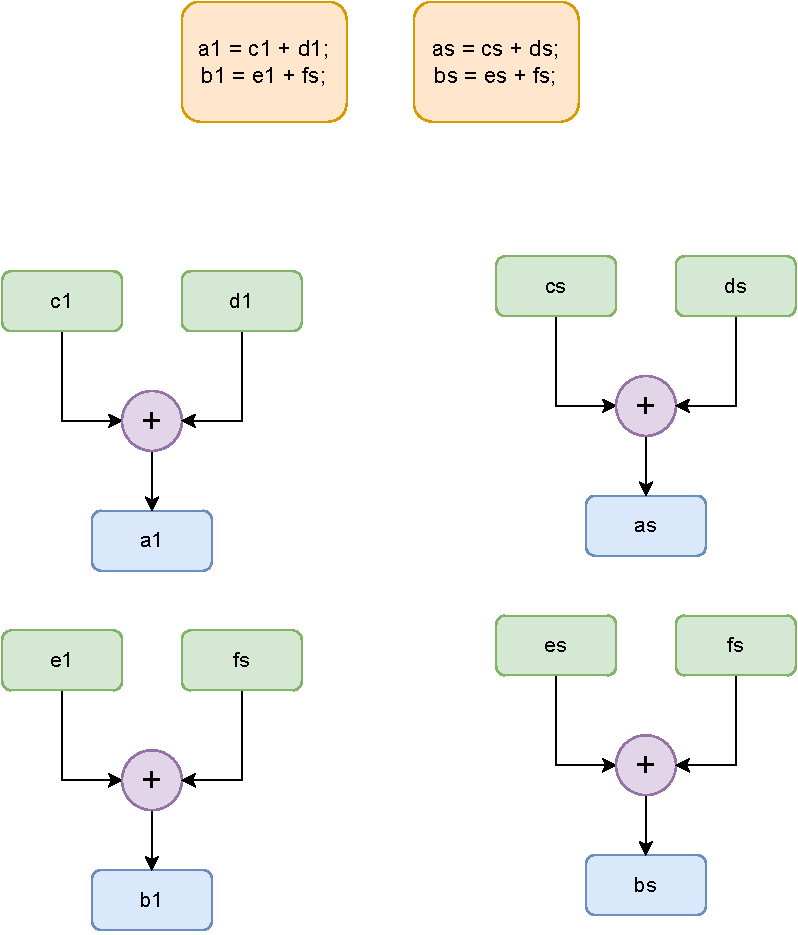
\includegraphics[scale=0.4]{FineGrainedMerge.pdf}
        \end{figure}

    \end{frame}

    \begin{frame}{Pending}

        \begin{itemize}
            \item Global Analysis to identify best merging combination. 
            \item Implement Redundant R/W elimination to improve scheduling (identified how to implement this)
            \item Graphs of relevance summarizing all 4096 examples and the effect of merging different ways.
        \end{itemize}

    \end{frame}

\end{document}